The goal of this work is to reduce the effort required to produce high-quality gaze animation modeling the gaze behavior as an automatically inferrable, easily editable sequence of gaze instances. %In this section, we present two evaluations we conducted to gauge our success: the first evaluation measured the authoring effort required to author and edit gaze using our approach in comparison with a traditional tool
We conducted a three-part evaluation of our approach. The first experiment assessed the amount of effort required to author gaze animations to confirm that our approach does indeed save animator time and effort. The second experiment assessed the subjective quality of the resulting animations to ensure that sufficient quality is achieved. The third experiment evaluated the effects of gaze editing on viewers' understanding of the scenario to show that the our approach allows animators to tell a new story through changes in the characters' attending behaviors.

\subsection{Authoring Effort}
\label{sec:GazeAuthoringEffortEvaluation}

We evaluated authoring effort in two ways. First, we investigated the effort required to add eye animation to a captured body motion without modifying the motion itself---something our tool can do automatically. We had two experienced animators add eye movements to seven scenarios, originally captured for the gaze inference evaluation (Section ~\ref{sec:GazeInference}), with a cumulative length of 2:36 minutes. Both animators used Autodesk MotionBuilder, where they set up a simple eye animation rig, which they keyed to create the desired eye movements. We measured authoring effort using two metrics: (1) time taken and (2) number of keys set. We found that the animators required on average 25 minutes and 86 keys per minute of animation. By contrast, our system can synthesize an equivalent amount of eye animation automatically, requiring on average 90 seconds of computation per minute of animation.

Second, we assessed the effort required to edit gaze animation in a scenario which already contained eye movements. An experienced animator was instructed to make the following edits: (1) introduce gaze aversion in a two-character interaction scenario (HandShake), (2) remove gaze toward an object in an environment interaction scenario (StealGem), (3) introduce gaze toward a new character in a multi-character interaction scenario (DrinkSoda), and (4) introduce gaze toward the camera in an environment interaction scenario (MakeSandwich). The edits in all the scenarios involved changing not just eye movements, but also head and (in some cases) torso pose. To accomplish the edits, the animator used layering and keyframing features in MotionBuilder. Meanwhile, a novice animator authored the same edits using our gaze editing tool. As before, we measured the time taken and number of operations required. For MotionBuilder, the latter is equivalent to the number of keys set, while for our tool, it refers to the editing operations discussed in Section~\ref{sec:GazeEditing}. The results, reported in Table~\ref{tab:GazeEditingEffortResults}, suggest equivalent edits may be achievable using our approach in 1/3 of the time and with 1/3 the number of operations required by traditional motion editing.
%
\begin{table}
\centering
\def\arraystretch{1.5}
\begin{tabular}{|l||l|l|l|l|}
\hline
\textbf{Scenario} & \multicolumn{2}{l|}{\textbf{Traditional}} & \multicolumn{2}{l|}{\textbf{Our Approach}} \\
\cline{2-5}
& Time & \# keys & Time & \# ops  \\
\hline
HandShake & 10:40 & 19 & 3:11 & 8 \\
StealGem & 1:29 & 9 & 1:30 & 4 \\
DrinkSoda & 9:05 & 43 & 3:51 & 9 \\
MakeSandwich & 10:43 & 33 & 4:05 & 13 \\
\hline
\end{tabular}
\caption{Gaze editing effort: traditional vs. our approach.}
\label{tab:GazeEditingEffortResults}
\end{table}

\subsection{Animation Quality}
\label{sec:GazeAnimationQualityEvaluation}

To evaluate the effect of our gaze authoring approach on perceived quality of produced animation, we conducted an experiment with human participants. We compared our approach to other methods of gaze animation production: no eye animation, eye movements recorded using an eye tracker, and hand-authored gaze. We showed participants pairs of videos of a motion-captured character performing various actions and asked them to choose the one they thought had superior animation. The videos in each pair were identical in every way except the gaze animation method. Different methods corresponded to the following study conditions: (1) \emph{no gaze}, (2) \emph{recorded gaze} (using an eye tracker), (3) \emph{hand-authored gaze}, and (4) \emph{synthesized gaze} (our approach.)

\subsubsection{Hypotheses}

We hypothesized the following: (1) \emph{Synthesized gaze} would be preferred over \emph{no gaze}. (2) \emph{Synthesized gaze} would be preferred over \emph{recorded gaze}. (3) \emph{Synthesized gaze} would be seen as equivalent to \emph{hand-authored gaze}. Hypothesis 2 is motivated by the consideration that raw eye-tracking data is noisy, non-trivial to map to an animated character, and often incorrect with respect to scenario requirements. Hypothesis 3 reflects the expectation that our approach can synthesize gaze animation at a level of quality approaching hand-authoring.

\subsubsection{Design}

The experiment involved three separate studies, each of which tested one of the hypotheses. Each study consisted of five task trials and followed a within-participants design, wherein the participants were asked to choose between videos in \emph{synthesized gaze} and one of the other conditions. Video pairs were presented to the participants in a randomized order.

\subsubsection{Stimuli}

Experiment stimuli were $5 \times 4$ video clips (five scenarios, each in four conditions) of a character animated using motion capture, 9 to 14 seconds in length. We created the \emph{no gaze} condition videos by extracting segments from the original scenarios created for the gaze inference evaluation (Section~\ref{sec:GazeInference}.) The scenarios were: ChatWithFriend, MakeSandwich, StackBoxes, StealGem, WalkCones. The \emph{hand-authored gaze} condition was created by extracting those same segments from the scenarios created for the authoring effort evaluation, while the \emph{synthesized gaze} condition was the result of applying our gaze inference to the segments. To create the \emph{recorded gaze} condition, we generated eye animations directly from eye tracking data.

\subsubsection{Measures}

Our experiment had the following subjective measures: (1) perceived \emph{animator competence}, (2) \emph{realism}, and (3) \emph{communicative clarity}. The measures were implemented as binary-choice questions the participant answered on each task trial: (1) ``On which video did the animator do a better job?'' (2) ``In which video were the character\'s movements more realistic?'' (3) ``In which video did the character communicate more clearly what they were doing?''

\subsubsection{Participants}

We conducted the experiment online using Amazon Mechanical Turk crowdsourcing service. We recruited 24 participants for each study---a total of 72 participants. The participants were paid at the rate of \$6/hour.
% TODO: Did you collect any demographics? I think people will at least expect gender breakdown.

\subsubsection{Results}

Upon collecting our data, we conducted separate analyses for each study of the experiment. We aggregated all the participants' binary answers across all the scenarios and obtained, for each condition, the count of how many times it was chosen over its counterpart in each measure. Then we compared the counts using chi-square tests of goodness-of-fit. We followed the guidelines suggested by~\citet{julnes1989analysis} for establishing a ``no difference'' in comparisons, with alpha level of $0.25$ (i.e., $p > .25$) to control for Type II errors.
The results, shown in~\ref{fig:GazeAnimationQualityResults}, were as follows.

\begin{figure}
\centering
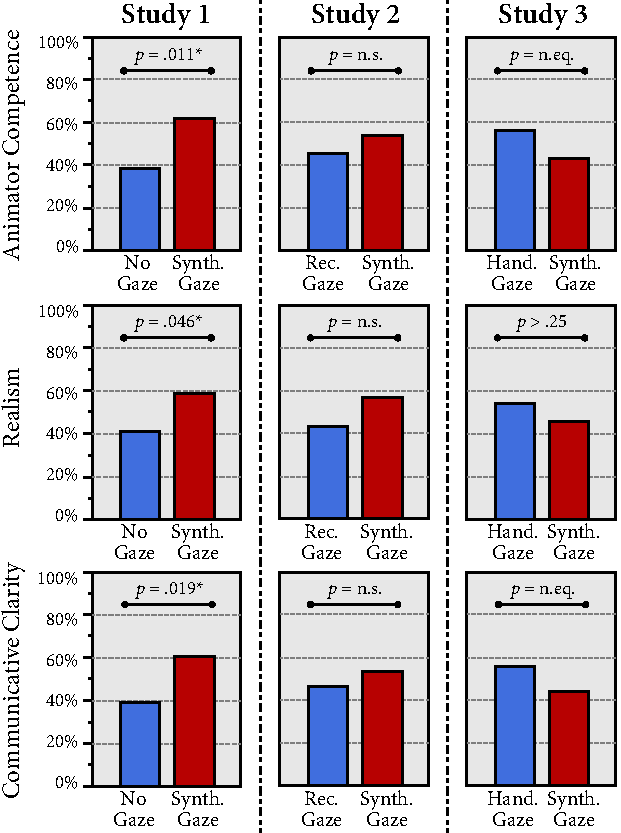
\includegraphics[width=0.8\textwidth]{gazeauthoring/Figures/StudyResults.pdf}
\caption{Results of the study comparing gaze animation produced using our approach (\emph{Synthesized Gaze}) to (1) no gaze animation, (2) gaze recorded using an eye tracker, and (3) hand-authored gaze. y-axis shows the percentage of trials in which one condition was chosen over the other.}
\label{fig:GazeAnimationQualityResults}
\end{figure}

The analysis of data from study one found a significant preference for \emph{synthesized gaze} over \emph{no gaze} on all measures: $\chi^2(1, 120) = 6.41, p = .011$ (animator competence), $\chi^2(1, 120) = 3.99, p = .046$ (realism), and $\chi^2(1, 120) = 5.54, p = .019$ (communicative clarity.) These results constitute support for Hypothesis 1.

Data from the second study showed that \emph{synthesized gaze} was not significantly preferred over \emph{recorded gaze} in any of the measures: $\chi^2(1, 120) = 0.83, p = .362$ (animator competence), $\chi^2(1, 120) = 2.12, p = .145$ (realism), and $\chi^2(1, 120) = 0.53, p = .466$ (communicative clarity.) Therefore, we did not find support for Hypothesis 2.

In study three, chi-square test results were the following: $\chi^2(1, 120) = 2.12, p = .145$ (animator competence), $\chi^2(1, 120) = 0.83, p = .362$ (realism), and $\chi^2(1, 120) = 1.63, p = .202$ (communicative clarity.) There was no significant difference in preference between \emph{synthesized gaze} and \emph{hand-authored gaze} on any of the measures. For the second measure (realism), the $p$-value exceeded the suggested equivalence margin of $p \geq .25$, indicating partial support for Hypothesis 3.

In a post-hoc exploratory analysis, we investigated the potential reasons for the lack of support for Hypothesis 2, as the findings contrasted our own observations. This analysis focused on how recorded and synthesized gaze differed across different scenarios. We found that scenario had a significant effect on participants' choice of \emph{recorded gaze} in all measures (e.g., $\chi^2(4, 55) = 25.04, p < .0001^*$ for the ``animator competence'' measure). Further inspection showed that scenarios with a close-up of the character benefited the most from our synthesized gaze approach, likely due to greater saliency of gaze cues. The differences between approaches were indiscernible in scenarios where the character's eyes were small on the screen and other motion components dominated. An illustrative example is the ChatWithFriend scenario, which was always chosen in \emph{synthesized gaze} condition over \emph{recorded gaze} in animator competence and realism measures, and 23 times out of 24 in communicative clarity.

Study results suggest that gaze animation is important for the perception of animation quality, and adding gaze animation using our approach leads to improvement in perceived animation quality. Benefits of gaze authoring may be more pronounced in scenarios where gaze behavior is perceptually dominant. Finally, we found evidence that the output of our method may be comparable in quality to gaze authored by a trained expert.

\subsection{Editing Effectiveness}
\label{sec:GazeEditingEffectEvaluation}

We conducted another experiment with human participants to evaluate the effectiveness of our gaze editing approach. We used our gaze editing tool (Section~\ref{sec:GazeEditing}) to edit the inferred gaze behavior in four scenarios. In each scenario, the character would spend a substantial portion of time focusing on a scene object or another character. We edited their gaze so they would focus more on another object or character instead. We showed the videos of each scenario to participants and had them estimate the amount of time the character focused on each object. The two versions of the video were identical in every way except the character's gaze behavior. We hypothesized that participants' estimates of the character's focus time would be significantly different in the edited scenario compared to the original scenario.

\subsubsection{Design}

The experiment followed a between-participants design to minimize transfer effects. There were two conditions: \emph{original gaze}, which showed the scenarios with inferred, unedited gaze behavior, and \emph{edited gaze}, which showed the scenarios with edited gaze behavior. In each condition, the participant would experience four trials of the task, one for each scenario. The scenarios were presented to the participants in a randomized order.

\subsubsection{Stimuli}

Experiment stimuli were $4 \times 2$ video clips (four scenarios, each in two conditions) of one or more characters animated using motion capture, 1 to 15 seconds in length. We created the \emph{original gaze} condition videos by extracting segments from the scenarios created for the gaze inference evaluation (Section~\ref{sec:GazeInference}.) The scenarios were: HandShake, MakeSandwich, DrinkSoda, StealGem. We added eye gaze animation to the scenarios using our gaze inference approach. Next, we created the \emph{edited gaze} condition videos by editing the gaze behavior of a character in each scenario. The edits involved introducing additional gaze shifts and fixations of another object or character, which is looked at infrequently or not at all in the original scenario. The following edits were performed:

\begin{enumerate}
\item \emph{HandShake} -- In the original scenario, the green character mostly looks at the blue character. In the edited scenario, we have the green character look down at the floor instead.
\item \emph{MakeSandwich} -- In the original scenario, the character looks either at the tabletop or off to the side. In the edited scenario, we have them sporadically look at the camera.
\item \emph{DrinkSoda} -- In the original scenario, the blue character mostly looks at the green character. In the edited scenario, we have the blue character look at the pink character as well.
\item \emph{StealGem} -- We introduced a second, yellow gem into this scenario for the purposes of the current experiment. In the original scenario, the character only looks down at the red gem. In the edited scenario, the character looks at the yellow gem instead of the red gem.
\end{enumerate}

\subsubsection{Measures}

The experiment had two objective measures per each scenario, for a total of 8 measures. The per-scenario measures were participants' estimates of the time spent by the character focusing one of two objects/characters in the scene. Each focus time was measured as percentage of the total time in the scenario. The participants specified their estimates on an 11-point scale, with items ranging from 0\% to 100\%.

For example, after viewing the DrinkSoda scenario (Figure~\ref{fig:GazeEditResults}), the participants answered the following two questions (each on an 11-point scale): ``How much was the blue character focusing on the green character?'' and ''How much was the blue character focusing on the pink character?''

\subsubsection{Participants}

We conducted the experiment online using Amazon Mechanical Turk crowdsourcing service. We recruited 24 participants or 12 per condition. The participants were paid at the rate of \$6/hour.

\subsubsection{Results}

We analyzed the data from each of our eight measures data using a two-tailed Student's t-test. The results, shown in~\ref{fig:GazeEditEffectResults}, were as follows.

\begin{figure}
\centering
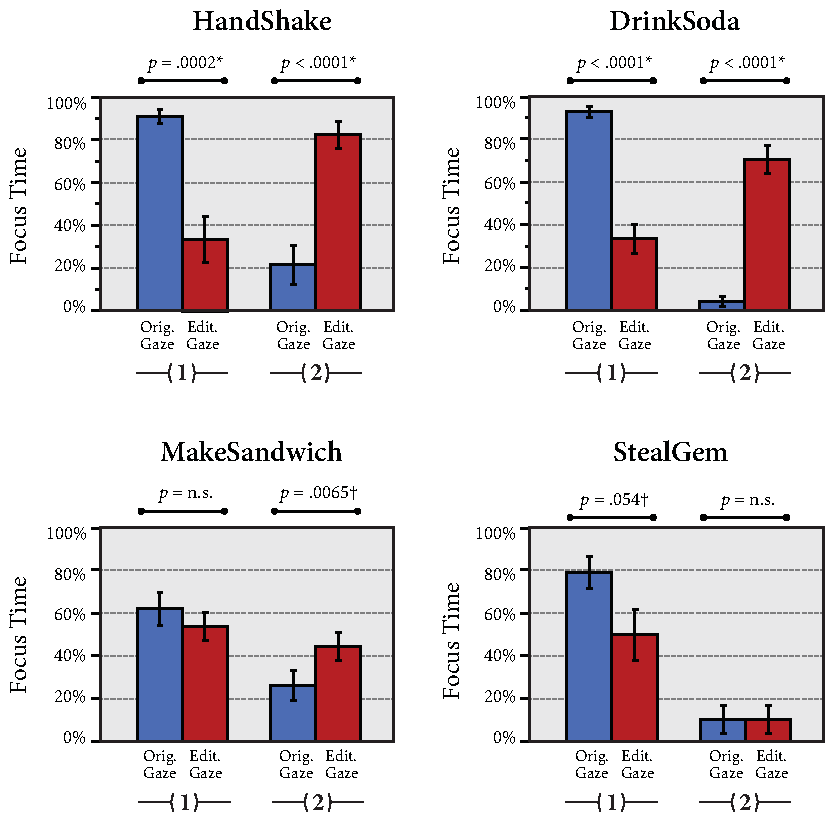
\includegraphics[width=1\textwidth]{gazeauthoring/Figures/StudyResults2.pdf}
\caption{Results of the study evaluating the effectiveness of our gaze editing approach. Each chart shows the participants' estimates of one character's focus times on two objects/other characters in the scenario, contrasted among the two conditions: \emph{Original Gaze} (gaze inference output) and \emph{Edited Gaze} (character's gaze edited using our tool.)}
\label{fig:GazeEditEffectResults}
\end{figure}

In the HandShake scenario, there was a significant difference in participants' estimates of focus time on the blue character, $t(13) = -5.10, p = .0002$. Likewise, there was a significant difference in their estimates of focus time on the floor, $t(20) = -5.49, p < .0001$.

In the MakeSandwich scenario, there was no significant difference in participants' estimates of focus time on the tabletop, $t(21) = -0.81, p = .4227$. However, participants in the \emph{edited gaze} condition did give marginally higher estimates for focus time on the camera than those in the \emph{original gaze} condition, $t(22) = 1.94, p = .0065$.

In the DrinkSoda scenario, there was a significant difference in participants' estimates of focus time on the green character, $t(13) = -8.27, p < .0001$, as well as their estimates of focus time on the pink character, $t(14) = 9.46, p < .0001$.

In the StealGem scenario, participants' estimates of focus time on the red gem were marginally lower in the \emph{edited gaze} condition than in the \emph{original gaze} condition, $t(18) = -2.06, p = .054$. There was no significant difference in their estimates of focus time on the yellow gem, $t(22) = 0, p = 1$.

Overall, these results suggest that our gaze editing approach is effective in that it allows a novice to modify the gaze animation of a character and obtain a scenario that is interpreted differently by na{\"i}ve viewers.
